\documentclass[12pt, a4paper]{article}

\usepackage[utf8]{inputenc}
\usepackage[french]{babel}
\usepackage[T1]{fontenc}
\usepackage{sistyle}
\usepackage{graphicx}
\usepackage{url}

\usepackage{listings}
\usepackage{color}
\definecolor{mygreen}{rgb}{0,0.6,0}
\definecolor{mygray}{rgb}{0.5,0.5,0.5}
\definecolor{mymauve}{rgb}{0.58,0,0.82}
\lstset{ %
  backgroundcolor=\color{white},   % choose the background color
  basicstyle=\footnotesize,        % size of fonts used for the code
  breaklines=true,                 % automatic line breaking only at whitespace
  captionpos=b,                    % sets the caption-position to bottom
  commentstyle=\color{mygreen},    % comment style
  escapeinside={\%*}{*)},          % if you want to add LaTeX within your code
  keywordstyle=\color{blue},       % keyword style
  stringstyle=\color{mymauve},     % string literal style
}

\usepackage[left=2.5cm,right=2.5cm,top=2.5cm,bottom=2.5cm]{geometry}

\bibliographystyle{plain}

\title{Programmation parallèle avec des Acteurs \\ \large{Projet de session INF7845 \\ UQAM}}
\date{\today}
\author{Antoine Laurent}

%\linespread{1.5}

\begin{document}
\maketitle
\newpage 

\section{Introduction}
la concurrence \\
Loi de moore \\
clock cycle \\
Différents languages \\

\section{Le modèle Acteur théorique}

Dans cette partie on va introduire ce que le modèle théorique des Acteurs, c'est à dire ce que sont les Acteurs et comment Hewitt à penser ce modèle quand il l'a introduit en 1973 \cite{hewitt1973session}. Pour cela on va voir la définition d'un Acteur, ce qu'ils peuvent faire comme action et leur encapsulation des données. Ensuite on regardera comment ils communiques entre eux et comment leur faire faire des actions. Puis on s'intéressera a comment les acteurs sont résistant aux pannes. Pour enfin voir le cycle de vie d'un Acteur.

\subsection{Qu'est ce qu'un Acteur}

Comme pour la programmation objet d'Alan Key ou tous est objet, les objets ont leur propre mémoire et qu'ils communiquent par message. Dans le modèle Acteur de Hewitt, tout est acteurs, les acteurs encapsulent leur état interne et ils communiquent par message. Hors les objets sont synchrone alors que les acteurs envoient les messages de manière asynchrone. 
\par 
Un acteur est donc une entité qui, à la réception d'un message peut: 
\begin{itemize}
\item Envoyer des messages a lui même ou a d'autres acteurs. Ces messages sont émis de manière asynchrone.
\item Changer de comportement : il effectue une action lié a ce message ou alors peut changer de comportement.
\item Créer un nombre fini de nouveaux Acteurs.
\end{itemize}
On verra après que l'habilité de l'Acteur d'être asynchrone, de pouvoir créer de nouveaux acteurs et de protéger son état interne permet de faire de la parallélisation très facilement et d'avoir une mise à l'échelle simplifié.

\subsection{Communication}

Comme dis plus haut les Acteurs communiquent entre eux par messages. Dans le modèle acteur, il n'y a pas de canaux de communications à établir comme un pipe pour les forks. Les acteurs communiquent d'eux même, soit par le réseaux si le système est distribué sur plusieurs machines, soit en interne lorsqu'ils sont présent sur la même machine. De plus la stratégie d'envoi de message est la technique du meilleur effort. Il n'y a pas de réémission , c'est à dire que lorsqu'un Acteur envoie un message a un autre, celui recevra le message au plus une fois. 
\par Ces messages sont adressé au différents Acteurs par leurs adresses. En effet un acteur peut être associé a une ou plusieurs adresses et on peut noter aussi que plusieurs Acteurs peuvent avoir la même adresse. Un bon exemple pour identifier cela est de penser au moteur de recherche Google, on connaît tous une seule adresse de Google, pourtant on n'effectue pas tous nos recherche sur le même serveur.
\par Les Acteurs ont une boite aux lettres, (mailbox) dans lesquelles ils reçoivent les messages qui leurs sont adressés. Cela marche un peut a la façon du système de poste si l'on veut s'en faire une image. Un acteur envoie un message et il est reçut dans la boite aux lettres de l'acteur concerné. Ils traitent alors un messages reçu à la fois.
\par Il est important aussi de noté que le temps que vas mettre un message a arriver a destination n'est pas connu. L'ordre d'arrivé des messages est donc complètement indéterminé. Ceci amène la propriété de l'indéterminisme au modèle Acteur. En effet si on reprend l'exemple de Hewitt \cite{video_hewitt}, on imagine qu'un acteur s'envoie à lui même un message <<go>> et un message <<stop>> comme décris figure \ref{fig1}. A la réception du message <<go>> l'acteur incrémente un compteur et à la réception du message <<stop>>, il arrête de compter. Étant donné que l'on ne sais pas combien de temps vont mettre les messages a revenir à l'acteur, et que ça ne dépend pas du système, le nombre obtenue a la réception du message <<stop>> est complètement aléatoire. Le modèle acteur à donc de l'indéterminisme.

\begin{figure}
\center
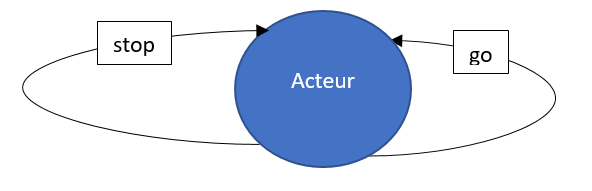
\includegraphics[scale=0.5]{actor_underminisism}
\caption{Exemple de l'indéterminisme du modèle Acteur.}
\label{fig1}
\end{figure}

\subsection{Concurrence avec les Acteurs}
Un des avantages principal du modèle Acteur est le fait qu'il introduit au programmeur de la concurrence à haut niveau. Dans le monde de la concurrence on peut retrouver deux manière de synchroniser les programmes, soit avec des états partagés comme les threads, soit avec des messages, comme pour les Acteurs \cite{haller2012actors}. Les threads peuvent devenir très vite difficile à programmer, à cause des verrous mortels, des courses à la donnée (data race). En effet ils utilisent des états partagés pour faire leurs calculs et cela oblige le programmeur a bien réfléchir a comment les threads vont communiquer et à quels moment protéger les variables partagées. Cela oblige a passé plus de temps à réfléchir à comment éviter les conflits entre les threads que de regarder la concurrence à un plus haut niveau. C'est à dire que l'application se déroule bien, de manière la plus efficace possible.

\par Les Acteurs eux ne possèdent pas d'états partagés, en effet chaque acteur a son propre état interne, et il ne doit pas communiquer d'état par messages par références aux autres acteurs ou à lui même. Car s'il faisait ça on retomberait sur un problème de verrous mortel ou de course à la donné. Le fait de communiquer par message empêche toute sorte de verrous mortel ou de course à la donné. En effet une course arrive lorsque deux threads accèdent a la même donné et au moins un des accès change la donné \cite{haller2012actors}. On ne peut pas avoir ça avec les système de messages, mais des courses à la donné de plus haut niveau peuvent arriver. Par exemple, on a vu qu'on ne sait pas l'ordre d'arrivé des messages, et dans le cas d'une transaction bancaire par exemple, si deux acteurs envoient un message a un troisième qui est la banque pour demander un retrait. Alors si la banque n'a assez d'argent que pour un seul des acteur, le premier message qu'elle va recevoir va avoir son argent alors que le deuxième non. Et cela indépendamment de l'ordre d'envoi des messages. 

\par De plus on peut voir que les acteurs sont beaucoup plus léger que les threads. Ils peuvent être plus facilement créer et détruit. On peut donc en créer beaucoup plus. De plus sur la JVM (Java Virtual Machine) par exemple, les threads sont des processus plus lourds car ils sont créer pour utiliser toute la puissance du processeur de la JVM. Et alors qu'on va pouvoir créer quelques millier de threads en parallèle sur la JVM, on va pouvoir y créer des millions d'acteurs. \cite{haller2012actors}.
\par Le fait de pouvoir créer plus facilement des acteurs que des threads, et en plus grand nombre, ainsi que de pouvoir étendre la puissance horizontalement (sur un réseau de machine), rend la mise à l'échelle très efficace comparé aux threads classiques. Un inconvénient de la concurrence par messages peut être la consommation importante que ça va engendrer au niveau du canal de communication.

\subsection{Tolérance aux pannes}
Le modèle Acteur à comme autre propriété d'être tolérant aux pannes, de la même façon qu'Erlang (qui est un langage de programmation basé sur le modèle Acteur) et sa philosophie <<Let it crash>>. Donc si un acteur venait à lancé une exception, il ne mettrait pas en danger tout le système, mais l'erreur serait alors envoyé a un superviseur qui déciderais de le relancer l'acteur, ou de l’arrêter.
\par Cela est possible car comme dis plus haut aucun acteur ne partage d'état avec d'autre acteurs du programme, il ne met donc pas en danger les autres acteurs lorsqu'il lui arrive une erreur.
\par on a donc chaque acteur qui est supervisé par un autre acteur appelé superviseur, mais on peut alors se demander : <<qui supervise le superviseur>>. L'idée est alors d'avoir une sorte de hiérarchie de superviseurs, qui vont chacun superviser un ou plusieurs superviseur de plus bas niveau, et ainsi pouvoir récupérer leurs erreurs. Au sommet de la hiérarchie ce trouverais le superviseur racine qui lui supervise le thread principal, comme par exemple Akka l'a implémenté \cite{akka}.

\subsection{Les Acteurs dans le monde actuel}
Aujourd'hui on peut retrouver des bibliothèque qui permettent d'implémenter le modèle acteur sur différents langages de programmation, comme Akka, Celluloid ou encore la bibliothèque Acteur de Nit. Bibliothèques que l'on verra dans la suite de ce documents. Mais il existe aussi des langages qui ont été créer par rapport à cette conception des acteurs. On peut retrouver Erlang qui est très orienté Acteur, mais ou on a pas chaque entité qui est un acteur, en effet il existe des types dur comme <<int>>, <<char>>, etc. On peut aussi parler d’Elixir, qui fait l'objet d'une étude pour de ce travail de session.
\par En plus des langages de programmations, le modèle acteur est utilisé dans le web et le cloud \cite{agha2014actors,vecchiola2009high}. Par exemple on peut citer l'application de message de Facebook qui était anciennement écrite en langage acteur, ou Twitter qui est développé en Scala, et dont le modèle de concurrence est un modèle acteur \cite{twitter_concurency}. Pour citer des projets plus récents, le service en ligne du jeu Halo 4 est implémenté en acteur, avec le framework Orleans développé par Microsoft.

\section{Différentes bibliothèques qui implémentent les Acteurs}
Dans cette partie on va regarder les trois bibliothèque suivante : Akka pour la JVM , Celluloid pour le langage Ruby et la bibliothèque Acteur de Nit. On va regarder comment utilisé les acteurs dans ces bibliothèques et comment elles implémentent le modèle Acteur. Plus tard dans le document on parlera des avantages et des faiblesses de chacune d'elles, mais cette partie est consacré à l'expérimentation des bibliothèques. 
\par Pour cela on va commencer par regarder la bibliothèque Akka, qui est la plus grosse des trois et permet de ce rapprocher le plus du modèle Acteur, ensuite on regardera Celluloid, qui permet d'apporter au Ruby l'aspect concurrence par Acteur. Et enfin on regardera la bibliothèque de Nit, qui est basée sur celle de Celluloid.

\subsection{Les acteurs en Scala avec Akka}
Akka est une bibliothèque qui apporte le modèle Acteur à la JVM. Dans le cadre de ce projet de session on va regarder seulement Akka pour le langage de programmation Scala, car il parait plus simple à première vue de programmer en acteur avec Scala qu'avec le langage Java. C'est une bibliothèque écrite en Scala et elle a pour but, en plus d'implémenter le modèle Acteur, de permettre au développeur de fournir un code plus simple, performant et fiable par rapport a la bibliothèque concurrente de base de Scala, ou de Java.

\subsubsection{Implémentation des Acteur par références}
Les acteurs dans Akka peuvent être désigner de deux manière différentes : par leur référence (\texttt{ActorRef})ou par leur chemin (\texttt{path}). Bien que les deux servent à désigner un acteur, les deux ne sont pas la même chose. 
\begin{itemize}
\item \textbf{Une référence :} c'est ce qui représente l'acteur créer et permet d'envoyer des messages a cet acteur. En effet lorsqu'on créer un acteur on obtient une référence qui est un sous type de \texttt{ActorRef}. On ne peut pas créer un acteur en utilisant l'opérateur \texttt{new}, mais on doit utiliser \texttt{Props} qui est une classe de configuration pour créer des acteurs. On peut voir la création d'un acteur dans la figure \ref{act_crea}.
\par Le fait de ne pas pouvoir instancier directement un acteur avec un \texttt{new} permet de garantir de manipuler un acteur et de gérer l'envoi de message. En effet il est alors impossible d'appeler une méthode que l'on définirait dans la classe de l'acteur. On a donc une abstraction qui permet de gérer avec ce qui semble de vrai acteurs. 
\item \textbf{Le chemin :} c'est le nom de l'acteur. Il est représenté par la suite successive de superviseur par lesquels on dois passer pour l'atteindre (sachant qu'un superviseur est le père de l'acteur). Le \texttt{path} est différent de la référence, en effet la référence désigne un seul acteur alors que la référence désigne un nom sous lequel il peut y avoir ou non un acteur.
\par Un \texttt{path} est local mais il peut aussi être un chemin a distance, par exemple le chemin de l'acteur de la figure \ref{act_crea} s'obtient par l'appel à la méthode \texttt{actor.path} est nous donne \texttt{akka://SimpleSystem/user/SimpleActor}. Un chemin à distance pourrait être \texttt{akka.tcp://my-sys@host.example.com:5678/user/service-b}
\newline
\end{itemize}
\par 
Pour créer les premiers acteurs dans Akka il faut avoir un système d'acteur, c'est lui qui va superviser les acteurs qui seront créer par lui. Pour créer un système d'acteur il suffit d'utiliser la fonction \texttt{ActorSystem("NomSystème")}. Ensuite chaque acteur que vous créer aura son propre contexte, et pourras créer des acteurs a partir de celui-ci. Il représente l'interface que l'on à avec l'acteur. 
\par Une fois que l'on a le système d'acteur, on peut créer et obtenir la référence sur l'acteur grâce à la méthode \texttt{actorOf()}. On peut alors commencer à envoyer des messages à cet acteur.

\begin{figure}[h]
\centering
\begin{lstlisting}[language=Scala]
__________________________________________________________________________
  class SimpleActor extends Actor {
    def receive = {
      case s:String => println("String : "+s)
      case i:Int => println("Int : "+i)
    }
    
    def foo = println("method foo")
  }
  val system = ActorSystem("SimpleSystem")
  val actor = system.actorOf(Props[SimpleActor], "SimpleActor")
  
  actor ! "Hello"
___________________________________________________________________________
\end{lstlisting}
\caption{Création d'un Acteur en Scala avec Akka}
\label{act_crea}
\end{figure}

\subsubsection{Tolérance aux pannes}
Dans cette partie, on va aborder la tolérance au pannes. On va regarder comment Akka implémente la philosophie <<Let it crash>>, quels sont les mécanismes et la philosophie employé. Pour cela on va voir qu'est-ce qu'un programme tolérant aux pannes devrait être capable de faire, et le comparer avec ce qu'Akka permet de faire. Ensuite on regardera comment Akka supervise les acteurs et les actions qu'ils peut prendre et le cycle de vie d'un acteur. Pour enfin s’intéresser aux stratégies utilisé par le superviseur pour savoir quelle action faire lorsqu'un type d'erreur survient.
\par Pour étudier la tolérance aux pannes dans cette partie on se base principalement sur la documentation officielle d'Akka \cite{akka} et le livre Akka in Action \cite{roestenburg2015akka}.

\par Tout d'abord on va rappeler ce que veut dire d'être tolérant aux pannes. Être tolérant aux pannes ne veut pas dire que qu'aucune exception ne doit arriver dans le système et que rien ne doit jamais tomber en panne. Au contraire, c'est de savoir que des pannes arrivent toujours, mais d'essayer de conserver le système en ligne sans avoir d'erreurs graves en essayant de récupérer ces pannes. Souvent lorsqu'une panne arrive, il est seulement important que les principales fonctionnalités d'un programme restent disponible, et on peut alors arrêter les plus petites si elles ont un problèmes, ou les mettre de coté pour trouver une solution plus tard. Si ces fonctionnalités sont trop importantes pour être arrêtées alors on il est possible d'avoir une sauvegarde de ces fonctionnalités pour pouvoir les remplacer directement.

\par Parlons maintenant des bonnes stratégies que l'on devrait avoir lorsqu'on parle d'un programme tolérants aux pannes. Ce comportement idéal est reporté du livre Akka in Action \cite{roestenburg2015akka} et ses caractéristiques sont décrites dans le tableau \ref{table1}.
\newline

\begin{table}[h]
\centering
\begin{tabular}{|l|p{.7\textwidth}|}
\hline
Isoler la faute & Une faute ne doit pas faire tomber en panne le système et doit être isolée pour cela.\\ \hline
Structure & Le système doit avoir une structure pour isoler les éléments en erreur des éléments actifs. \\ \hline
Redondance & On doit pouvoir avoir un composant de secoure quand le composant tombe en erreur.\\ \hline
Remplacement & On doit pouvoir remplacer un composant du système sans que les autres composants qui étaient en communication avec soient dérangés par ce changement. Ils doivent pouvoir communiquer avec le remplacement de la même façon qu'ils communiquaient avec l'ancien. \\ \hline
Redémarrage & On doit pouvoir redémarrer un composant à son état initial. \\ \hline
Cycle de vie & Les composant devront avoir un cycle de vie défini pour pouvoir être démarré, stoppé ou redémarré. \\ \hline
Suspension & Lorsqu'un composant est en erreur, les autres composants actifs doivent arrêter de communiquer avec. \\ \hline
Séparation du code & Le code pour l’exécution normale du programme ne doit pas être mélangé avec le code destiné au recouvrement de panne. \\ \hline
\end{tabular}
\caption{Caractéristiques pour un système tolérants aux pannes}
\label{table1}
\end{table}
\par On va maintenant s'intéresser à la gestion des pannes par Akka, pour pouvoir comparer avec le comportement idéal décrit dans la table \ref{table1}. Dans Akka le flux normal du programme est géré séparément du flux de recouvrement. Le flux normal correspond à l’exécution normale du programme, c'est à dire quand il n'y a pas d'erreur et le flux de recouvrement correspond à ce qui se passe quand l'acteur crash. Effectivement, les acteurs qui participent au flux normal sont juste programmés pour effectuer les taches du programme. Ils jouent leur rôle d'acteur, et ce sont les superviseurs de ces acteurs qui sont prévenus lorsqu'il y a une erreur sur un acteur qu'ils supervisent qui crash. 
\newline
\textbf{Général :}
\par Quand un acteur crash, on le laisse crasher, on n'attrape pas l'exception. Ça boite aux lettres est alors suspendu le temps que son superviseur choisisse une action à effectuer pour cet acteur. Le superviseur a alors 4 options vis à vis de l'acteur crashé :
\begin{itemize}
\item Redémarrer son subordonné, ce qui le fait revenir à son état initial.
\item Reprendre l’exécution du subordonné, il conserve alors son état interne.
\item Arrêter le subordonné.
\item Faire monter l'information lorsqu'il ne sait pas comment gérer l'erreur.
\end{itemize}
Lorsqu'on reprend l’exécution d'un acteur, on reprend l'exécution de tous les acteurs qu'il a créer. De même lorsqu'on redémarre cet acteur, on redémarre tous ces fils, en les ayants arrêté préalablement.
\par Chaque acteur est supervisé par l'acteur qui le créer. En effet Akka à choisit un modèle de supervision parentale. Il n'y a pas d'adoption, si un parent est arrêté alors tous ces enfants le sont aussi. Cela permet un arrêt propre de tout un arbre ou sous arbre d'acteurs.
\newline
\newline
\textbf{Cycle de vie :}
Comme on l'a vu plus haut, un acteur peut être démarrer, redémarré ou bien arrêté. C'est les trois types d’événements que l'on retrouve dans le cycle de vie d'un acteur dans Akka. Lors de l'arrêt d'un acteur, il ne peut plus recevoir de messages et il va se faire ramasser par le <<garbage collector>>.

\par On peut démarrer un acteur avec la méthode \verb!actorOf! qui est soit une méthode utilisé par le \verb!ActorSystem! si c'est un acteur créer dans le thread principal (un acteur de haut niveau). Soit une méthode utilisé par \verb!ActorContext! si c'est un acteur créer par un autre acteur du système. Une fois l'instance créer, la méthode \verb!preStart! est appelée, puis l'acteur est démarré. On peut utilisé cette méthode pour initialiser l'état de l'acteur.

\par On arrête un acteur en utilisant la méthode \verb!stop!, soit sur l'\verb!ActorSystem! ou sur l'\verb!ActorContext!. Comme pour le démarrage d'un acteur, avant qu'on termine l'acteur la méthode \verb!preStop! est appelée. 	 

\par Enfin l'acteur est redémarré de base lorsqu'il crash, on verra cela dans la partie Superviseur et Stratégie. Par exemple si on envoie l'exception \texttt{throw new IllegalStateException( "restart forcé")} alors le superviseur fera redémarrer l'acteur. Quand un acteur crash, on remplace l'acteur par un nouvel acteur et on l'attache à sa référence \verb!ActorRef!. L'acteur crashé ne reçoit pas de message \verb!Terminate!, on peut donc lui faire envoyer un message à lui même après le redémarrage. Ainsi le nouvel acteur recevra ce message puisque c'est lui qui est associé à l'\texttt{ActorRef}.
\newline
\newline
\textbf{Superviseur et Stratégies :}
Lorsque l'on démarre une application Akka, on démarre au moins trois acteur, qui forment une hiérarchie (figure \ref{fig2}): 
\begin{itemize}
\item Le root Guardian : c'est le superviseur de tous les acteurs de haut niveau. Il ne peut pas faire remonter de messages, il n'a pas de superviseur, ce n'est donc pas un vrai acteur. Il arrête ses fils  au moindre trouble \cite{akka}, et c'est lui qui arrête le système d'acteur.
\item Le user Guardian : c'est le superviseur de tous les acteurs créer par l'utilisateur. Si on éteint cet acteur, on éteint tous les acteurs de l'utilisateur.
\item Le system Guardian : c'est le superviseur de tous les loggers de l'application.
\newline
\end{itemize}

\begin{figure}
\centering
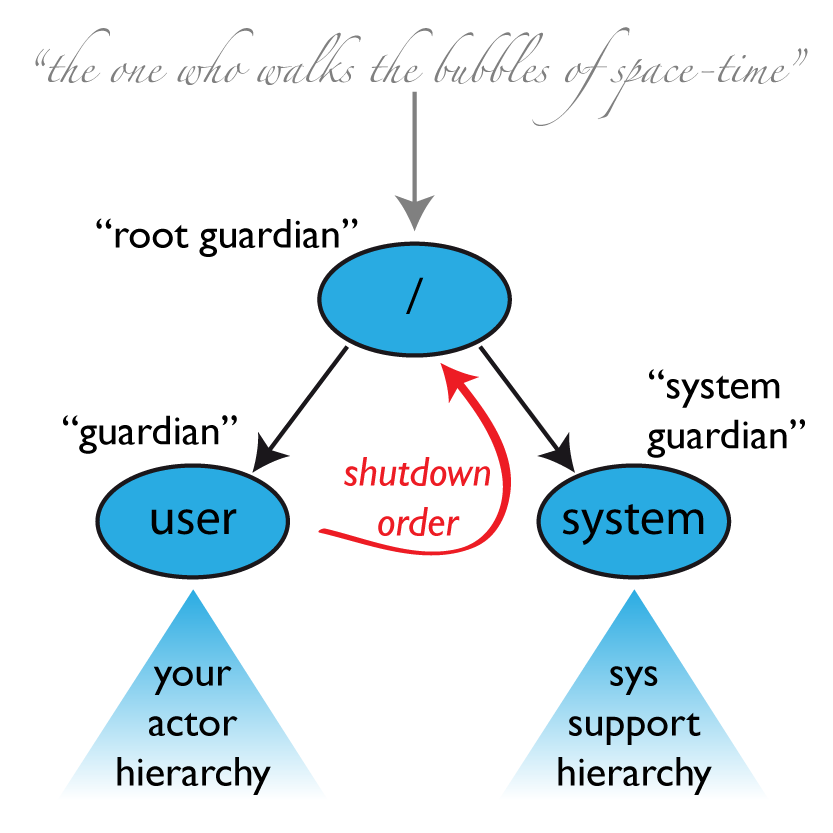
\includegraphics[scale=1]{guardians.png}
\caption{hiérarchie des trois superviseurs de plus haut niveau dans Akka \cite{akka}}
\label{fig2}
\end{figure}

\par Les acteurs qui supervisent ont une stratégie pour connaître  quelle action prendre quand une exception ce produit. Par défaut un superviseur va vouloir redémarrer l'acteur en question pour tous type d'exception qui a produit le crash de l'acteur. Les seuls cas ou il ne va pas essayer de redémarrer son fils et si l'erreur survient lors de l'initialisation de l'acteur ou lorsque celui-ci à été tué.
\par Cette stratégie peut être changé si on veut en redéfinissant la méthode \texttt{supervisorStrategy}. On peut voir un exemple de redéfinition figure \ref{fig3}.

\begin{figure}[h!]
  \begin{lstlisting}[language=scala]
  __________________________________________________________________________
  import akka.actor.OneForOneStrategy
  import akka.actor.SupervisorStrategy._
  import scala.concurrent.duration._

  override val supervisorStrategy =
      OneForOneStrategy(maxNrOfRetries = 10, withinTimeRange = 1 minute) {
        case _: ArithmeticException => Resume
        case _: NullPointerException => Restart
        case _: IllegalArgumentException => Stop
        case _: Exception => Escalate
  __________________________________________________________________________
  \end{lstlisting}
  \caption{Changement de stratégie pour un superviseur \cite{akka}}
  \label{fig3}
\end{figure}
\par On peut voir ici qu'on utilise la stratégie \texttt{OneForOneStrategy}, cela signifie qu'on différencie tous les fils lorsqu'on reçoit une exception de l'un deux. Les autres acteurs supervisé par l'acteur ne sont pas concerné par le destin de celui qui à crashé. Au contraire la stratégie \texttt{AllForOneStrategy} associe le même destin à tous les acteurs qu'il supervise. Si un acteur crash et que le superviseur le tue, alors tous les acteurs sont arrêtés.
\newline
\newline
\textbf{Monitoring :}
\par Un acteur ne peut pas être superviseur d'un autre acteur qu'il n'a pas créer, mais il peut être son moniteur grâce à la méthode \texttt{watch(ActorRef)}, qui est appelée sur l' \texttt{ActorContext}. Ainsi lorsque l'acteur est arrêté, le moniteur reçoit un message lui disant que l'acteur qu'il regardait s'est arrêté. C'est une des raisons pour laquelle il ne peuvent pas tuer un acteur lorsqu'il le redémarre car sinon un acteur qui était son moniteur ne pourrait pas savoir s'il a été redémarré ou arrêté.
\newline
\par 
On a donc pu voir que Akka permet de respecter complètement les bonnes stratégies pour la tolérances aux pannes. En effet, on peut isoler la faute, pour cela un superviseur a juste à terminer l'acteur. On peut remplacer un acteur sans que le système soit affecter, ce qui implique une structure pour gérer l'acteur erroné et un remplacement fonctionnel. Cela convient aussi pour la redondance, en effet si un acteur peut être remplacé il peut alors être remplacé par une sauvegarde de lui même. Un acteur a un cycle de vie et peut être suspendu. Enfin il le code application est défini indépendamment du code pour la récupération d'erreurs.
\subsubsection{Messages et Boite aux lettres}
Akka nous donnes des références sur des acteurs, et on peut envoyer des messages a ces références via la méthode \texttt{tell(message, ActorRef)} ou alors plus simplement avec le \texttt{!} comme montrer dans la figure \ref{act_crea}. Lorsqu'un acteur reçoit un message, il est réceptionné dans sa boite aux lettres, qui est implémenté comme une FIFO. Chaque acteur à généralement ça propre boite aux lettres, mais dans certains cas un groupe d'acteurs peut avoir la même boite aux lettres (voir BalancingPool \cite{akka}). De plus cette boite aux lettre peut être configuré sur plusieurs critères, elles peut être par exemple bloquer l'arrivé de nouveau messages si celle-ci est pleine, ou être partagée entre plusieurs acteurs comme énoncé ci-dessus.
\par Lorsqu'un acteur reçoit un message il fait ce qu'on appelle du message matching pour voir s'il a une action spécifiée à la réception de ce messages. On peut voir par exemple dans la figure \ref{act_crea} que l'acteur sais comment réagir aux String et aux Integers. On peut aussi, dans le but de rendre l'application <<plus Acteur>>, créer des cas de messages en créant de objet Scala, comme on peut le voir dans la première ligne de la figure \ref{cas_mesg}.
\par Lorsqu'un message est envoyé mais ne peut pas joindre la destination parce que par exemple l'acteur est terminé, le messages va dans ce qu'appelle Akka les DeadLetters, c'est une boite aux lettres où sont redirigés les messages qui ne peuvent pas être délivrés.
\par Akka, comme dans le modèle théorique n'assure pas la réception du message. En effet il sera reçut au plus une fois par le destinataire. Par contre Akka assure que si plusieurs messages sont envoyé a un acteurs par l'envoyeur successivement, alors les messages seront reçus dans le même ordre que celui de l'envoie. Par exemple si A envoi à B m1, m2 et m3, alors si B reçoit m1, ce sera forcément avant m2 et m3.
\newline

\begin{figure}[h]
\centering
\begin{lstlisting}[language=scala]
__________________________________________________________________________
case object AskNameMessage

class SimpleActor extends Actor {
  import context._
  implicit val timeout = Timeout(FiniteDuration(1, TimeUnit.SECONDS))
  
	def receive = {
	  case AskNameMessage => sender ! "Antoine"
	  case _ => context.actorSelection("akka://SimpleSystem/user/SimpleActor2").resolveOne().onComplete {
	    case Success(actorRef) => actorRef ! "coucou"
	    case Failure(ex) => println("user/" + "somename" + " does not exist")
	  }
	}
}
__________________________________________________________________________
\end{lstlisting}
\caption{Exemple de cas de messages et réception de tous messages en Scala avec Akka}
\label{cas_mesg}
\end{figure}

\par En plus de pouvoir envoyer un message de manière asynchrone avec la méthode \texttt{tell(...)}, Akka permet d'enregistrer ce messages dans un Future avec la méthode \texttt{ask(mesg, Actorref)} ou encore \texttt{?}. Cela permet d'envoyer un message et d'attendre pour une réponse sans bloquer le le thread principal. On peut ensuite récupérer ce résultat de manière bloquante, i.e en attendant que le future ai fini son exécution ou alors avec la commande \texttt{onComplete()}. On peut voir un exemple d'utilisation des futurs dans  la figure \ref{futur}
\newline 

\begin{figure}[h]
\centering
\begin{lstlisting}[language=scala]
__________________________________________________________________________
object future extends App {

	val system = ActorSystem("SimpleSystem")
	val myActor = system.actorOf(Props[SimpleActor], name = "myActor")

	implicit val timeout = Timeout(5 seconds)
	val future = myActor ? AskNameMessage
	val result = Await.result(future, timeout.duration).asInstanceOf[String]
	println(result)

	system.terminate()

}
__________________________________________________________________________
\end{lstlisting}
\caption{Exemple d'utilisation de Future dans Scala avec Akka}
\label{futur}
\end{figure}

\par Enfin on peut parler des routeurs qui permettent dans Akka d'implémenter le fait que plusieurs acteurs aient la même adresse. Ce n'est pas a proprement parler plusieurs acteurs avec la même adresse. On a un Routeur, qui est un acteur avec une adresse, ce routeur créer un Pool d'acteurs et lorsqu'il va recevoir un message, va pouvoir l'envoyer aux autres. La manière dont il l'envoi (broadcast, etc) dépend du protocole de routage qu'on lui demande d'implémenter.

\subsubsection{Autres fonctionnalités d'akka}
Akka est une très grande bibliothèque dans laquelle il existe beaucoup d'autres fonctionnalités. J'ai choisi ici d'essayer de présenter les fonctionnalités les plus importantes pour un système d'acteur mais aussi de comprendre comment elles ont été faites. Mais Akka est tellement large qu'on pourrait y consacrer un projet de session entièrement. Néanmoins je voulais mentionner quelques autres fonctionnalités, comme les clusters, la gestion de HTTP pour des applications Client Serveur, Actor DSL qui est une manière plus simple et rapide de faire de la programmation acteur. Toutes ces fonctionnalités peuvent être retrouvées dans la documentation d'Akka \cite{akka}.

%\subsection{Les acteurs en Ruby avec Celluloid}
%Dans cette partie 
%\subsubsection{Implémentations des acteurs}

%\subsubsection{Les Pools}

%\subsubsection{Tolérance aux pannes}

%\subsubsection{Cycle de vie}

\subsection{Les acteurs en Nit avec la bibliothèque d'acteur}

\subsubsection{Implémentations des acteurs}


\section{Les avantages et faiblesses de ces bibliothèques}

\subsection{Akka}

\subsection{Nit}


\section{Programme réalisé}
Chat avec des acteurs  : IO\\
Mandelbrot ? : CPU\\

\section{Conclusion}

\bibliography{references.bib}
\end{document}